\documentclass{standalone}
\usepackage{xcolor}
\usepackage{forest}
\usepackage{tikz}
\begin{document}
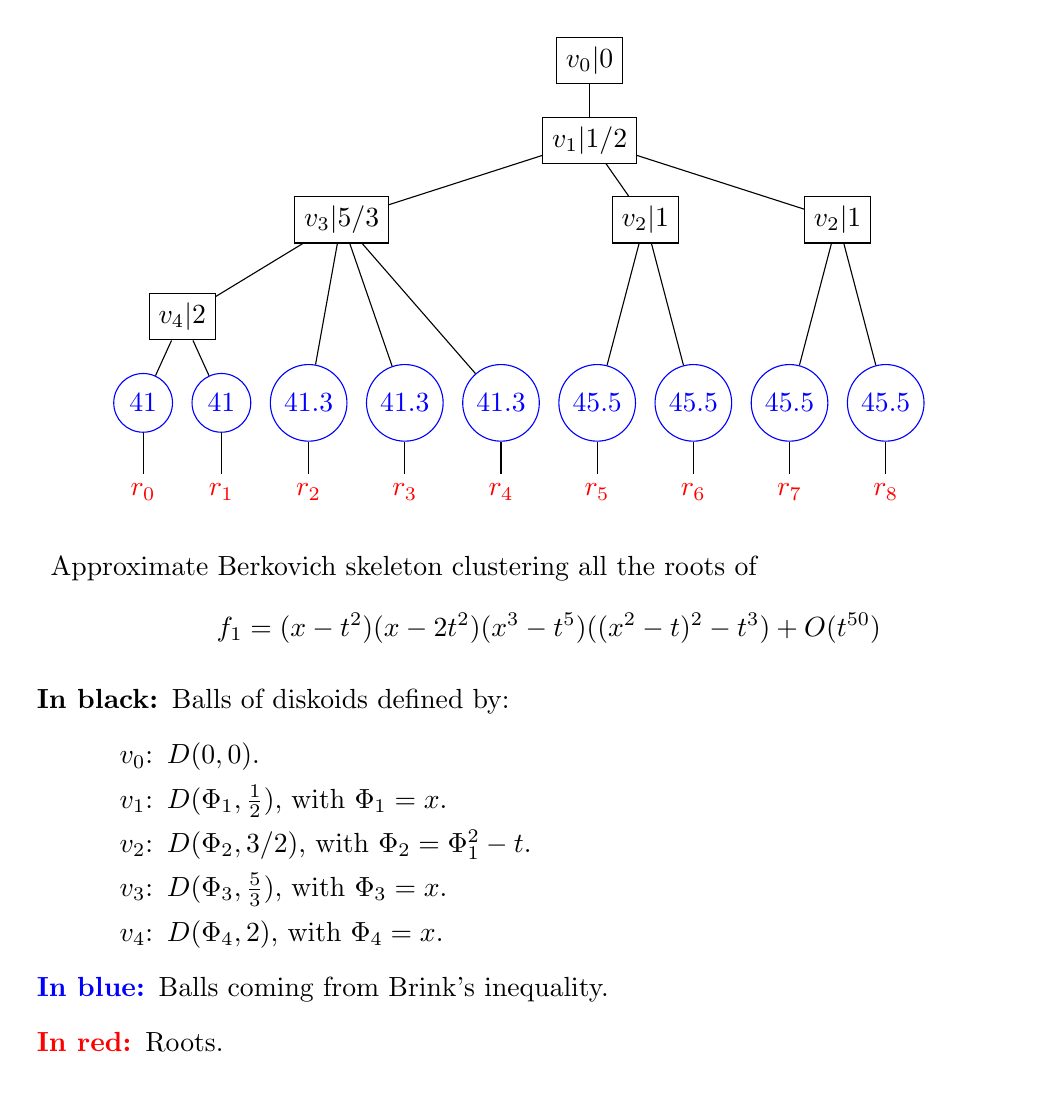
\begin{tikzpicture}
\node[anchor=north] (tree) at (0,0) {
\begin{forest}
[$v_{0} \vert 0$, draw,  black[$v_{1} \vert 1/2$, draw,  black[$v_{3} \vert 5/3$, draw,  
black[$v_{4} \vert 2$, draw,  black[$41$, circle, draw,  blue, tier=Brink[$r_{0}$,  red, tier=root]
]
[$41$, circle, draw,  blue, tier=Brink[$r_{1}$,  red, tier=root]
]
]
[$41.3$, circle, draw,  blue, tier=Brink[$r_{2}$,  red, tier=root]
]
[$41.3$, circle, draw,  blue, tier=Brink[$r_{3}$,  red, tier=root]
]
[$41.3$, circle, draw,  blue, tier=Brink[$r_{4}$,  red, tier=root]
]
]
[$v_{2} \vert 1$, draw,  black[$45.5$, circle, draw,  blue, tier=Brink[$r_{5}$,  red, tier=root]
]
[$45.5$, circle, draw,  blue, tier=Brink[$r_{6}$,  red, tier=root]
]
]
[$v_{2} \vert 1$, draw,  black[$45.5$, circle, draw,  blue, tier=Brink[$r_{7}$,  red, tier=root]
]
[$45.5$, circle, draw,  blue, tier=Brink[$r_{8}$,  red, tier=root]
]
]
]
]
\end{forest}
};
\node[anchor=north, align=center] at (tree.south) {
    \parbox{\linewidth}{%
        \centering
        \begin{description}
        	\item[] Approximate Berkovich skeleton clustering all the roots of  \[f_1=(x-t^2)(x-2t^2)(x^3-t^5)((x^2-t)^2-t^3)+O(t^{50})\]
            \item[In black:] Balls of diskoids defined by:  
                \begin{itemize}
                    \item[ $v_{ 0 }$:] $D(0,0)$.
                    \item[ $v_{ 1 }$:] $D(\Phi_1,\frac{1}{2})$, with $\Phi_1=x$.
                    \item[ $v_{ 2 }$:] $D(\Phi_{2}, 3/2)$, with $\Phi_{2}=\Phi_{1}^{2} - t$.
                    \item[ $v_{ 3 }$:] $D(\Phi_3,\frac{5}{3})$, with $\Phi_3=x$.
                    \item[ $v_{ 4 }$:] $D(\Phi_4,2)$, with $\Phi_4=x$.
                \end{itemize}
            \item[\textcolor{blue}{ In blue:}] Balls coming from Brink's inequality.
            \item[\textcolor{red}{In red:}] Roots.
        \end{description}%
    }
};
\end{tikzpicture}
\end{document}